\section{Theorie}
\label{sec:Theorie}

\subsection{Zielsetzung}
\label{subsec:Zielsetzung}
Ziel dieses Versuchs ist es, mit Hilfe der sogenannten
Debye-Scherrer-Methode die Struktur einer Kristallprobe
zu bestimmen und die Gitterkonstante zu messen.

\subsection{Allgemines}
\label{subsec:allgemein}

Festkörper wie zum Beispiel Salze und Metalle
sind aus periodischen
Kristallstrukturen zusamengesetzt. Dabei sind im
Allgemeinen die einzelenen Kristallite zufällig
ausgerichtet. Wenn ein solcher Festkörper untersucht wird,
wird nur das statistische Mittel der Kristalle beobachtet.
Zur Untersuchung der Eigentlichen Kristallstruktur
können somit nur einzelne Kleinkristalle bzw.
Einkristalleverwendet werden.


\subsection{Kristallgitter}
\label{subsec:kristallstrukturen}
Um die Periodischen Atomstrukturen eines Kristalls
zu beschreiben, wird ein Punktgitter verwendet.
Jedem Gitterpunkt wird eine festgelegte Atomgruppierung,
die sogenannte Basis, zugeordnet.
Es existieren theoretisch unendlich viele solcher Punktgitter.
Jedes wird durch drei sogenannte Translationsvektoren
$\vec{x}_{1}$, $\vec{x}_{2}$, $\vec{x}_{3}$ gekennzeichnet.
Durch Linearkombination dieser Vektoren lässt sich
jeder Gitterpunkt
\begin{align}
  \label{eqn:1*}
  \vec{t} = n_{1} \vec{x}_{1} + n_{2} \vec{x}_{2} + n_{3} \vec{x}_{3}
\end{align}
beschreiben.
Mit Hilfe des durch die drei Vektoren $x_{i}$ aufgespannten
Parallelepipeds(siehe Abbildung \ref{fig:abb2}) lässt sich die
kleinstmögliche strukturbestimmende Einheit des Gitters,
die sogenannte Elementarzelle, erhalten.
Dabei wird zwischen primitiven und nichtprimitiven Einheitszellen
unterschieden. Im Fall einer primitiven Einheitszelle,
liegen auf den Eckpunkten des Parallelepipeds Atome.
Ist dies nicht der Fall, handelt es sich um eine
nichtprimitive Einheitszelle.\\ \\
Die verschiedenen Punktgitter werden anhand ihrer Symmetrie
in 14 als \textit{Bravais-Gitter} bezeichnete Arten eingeteilt.
Diese lassen sich in 7 Gruppen zusammenfassen.
\subsubsection{Kubische Kristallstrukturen}
\label{subsubsec:kubische_gitter}

Die Gitterstruktur von vielen in der Natur vorkommenden Elementen,
sind häufig gegeben durch die sogenannten Kubischen Gitter.
Bei kubischen Gittern sind besitzen die drei Translationsvektoren
alle die selbe Länge und stehen jeweil senkrecht aufeinander.\\
Es wird zwischen \textit{kubisch-primitiven},
\textit{kubisch-flächenzentrierten} und
\textit{kubisch-raumzentrierten Gittern} unterschieden. \\ \\
Das \textit{kubisch-primitive Gitter}(siehe Abbildung \ref{fig:sc})
kennzeichnet sich dadurch,
das die Atome der Einheitszelle auf den Ecken
eines Würfels platziert sind. Somit kann als Basisvektor trivial
der Nullvektor angegeben werden.\\ \\
Das \textit{kubisch raumzentrierte Gitter}(siehe Abbildung \ref{fig:bcc})
gleicht dem primitiven, allerdings befindet sich noch
zusätzlich ein Atom im Mittleren des Würfels.
Somit besteht in diesem Fall die Basis aus zwei Atomen.
Diese Basisvektoren sind durch:
\begin{align}
  \label{eqn:2*}
  \begin{pmatrix}
    0, 0, 0;
  \end{pmatrix}\\
  \begin{pmatrix}
    \frac{1}{2}, \frac{1}{2}, \frac{1}{2};
  \end{pmatrix}
\end{align}
gegeben.\\ \\

\begin{figure}[hhh]
  \centering
  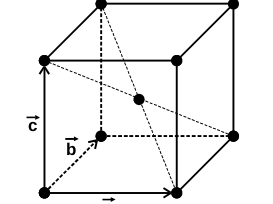
\includegraphics[width=0.9\textwidth]{abbildungen/bcc.png}
  \caption{Einheitszelle des kubisch-raumzentrierten Gitters.[\cite{sample}]}
\end{figure}

Das \textit{kubisch flächenzentrierte Gitter} gleicht dem
\textit{kubisch-primitiven}, hat
allerdings zusätzlich jeweils auf den Mitten der Würfelflächen Atome.
Die Basisvektoren sind durch
\begin{align}
   \label{eqn:3*}
   \begin{pmatrix}
     0, 0, 0;
   \end{pmatrix}\\
   \begin{pmatrix}
     \frac{1}{2}, \frac{1}{2}, 0;
   \end{pmatrix}\\
   \begin{pmatrix}
     \frac{1}{2}, 0, \frac{1}{2};
     \end{pmatrix}\\
     \begin{pmatrix}
       0, \frac{1}{2}, \frac{1}{2};
     \end{pmatrix}
\end{align}
gegeben.

\begin{figure}[hhh]
  \centering
  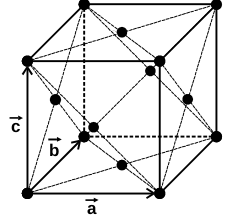
\includegraphics[width=0.9\textwidth]{abbildungen/fcc.png}
  \caption{Einheitszelle des kubisch-raumzentrierten Gitters.[\cite{sample}]}
\end{figure}

Durch Verschiebung des \textit{kubisch-flächenzentrierten Gitters}
um eine viertel Raumdiagonale ergibt sich die sogenannte
\textit{Diamant-Struktur}(siehe Abbildung \ref{fig:diamant}).
Die zugehörigen Basisvektoren sind gegeben durch die
Basisvektoren des \textit{kubisch-flächenzentrierten Gitters}
und zusätzlich durch die Vektoren:
\begin{align}
   \label{eqn:4*}
   \begin{pmatrix}
    \frac{1}{4}, \frac{1}{4}, \frac{1}{4}
  \end{pmatrix}\
  \begin{pmatrix}
    \frac{3}{4}, \frac{3}{4}, \frac{1}{4}
  \end{pmatrix}\
  \begin{pmatrix}
    \frac{3}{4}, \frac{1}{4}, \frac{3}{4}
  \end{pmatrix}\
  \begin{pmatrix}
    \frac{1}{4}, \frac{3}{4}, \frac{3}{4}
  \end{pmatrix}
\end{align}

\subsection{Kristallstrukturen aus zwei Atomarten}
\label{subsec:2atome}
Die bisher diskutierten Kristallstrukturen sind alle aus nur
einem Atomtyp zusammengesetzt. Im Folgenden wird auf Strukturen
eingegangen, die aus zwei verschiedenen Atomtypen bestehen.\\ \\
Die sogeannte \textit{Zinkblende-Struktur} entsteht aus der
in \ref{subsec:kubische_gitter}
aufgeführten Diamantstruktur, indem an den Stellen der zum
kubisch-flächenzentrierten verschiedenen Vektoren der Einheitszelle
ein anderer Atomtyp auftritt.\\
Bei der \textit{Steinsalz-Struktur}(siehe Abbildung \ref{fig:steinsalz})
sind die verschiedenen Atomtypen
jeweils in zwei kubisch-flächenzentrierten Gittern angeordnet, die um eine
halbe Raumdiagonale zueinander verschoben sind. Die Atompositionen
in der Einheitszelle sind:
\begin{align}
  \label{eqn:5*}
  \text{Atom }(1) :&
  \begin{pmatrix}
    0, 0, 0
  \end{pmatrix}\
  \begin{pmatrix}
    \frac{1}{2}, \frac{1}{2}, 0
  \end{pmatrix}\
  \begin{pmatrix}
    \frac{1}{2}, 0, \frac{1}{2}
  \end{pmatrix}\
  \begin{pmatrix}
    0, \frac{1}{2}, \frac{1}{2}
  \end{pmatrix}\\
  \label{eqn:6*}
  \text{Atom }(2) :&
  \begin{pmatrix}
    0, 0, 0
  \end{pmatrix}\
  \begin{pmatrix}
    1, 1, \frac{1}{2}
  \end{pmatrix}\
  \begin{pmatrix}
    1, \frac{1}{2}, 1
  \end{pmatrix}\
  \begin{pmatrix}
    \frac{1}{2}, 1, 1
   \end{pmatrix}
\end{align}
Die sogenannte \textit{Cäsium-Chlorid-Struktur}(siehe Abbildung \ref{fig:cscl})
ensteht, wenn zwei \textit{kubisch-primitive Gitter}, mit jeweils
unterschiedlichen Atomen, um eine halbe Raumdiagonale zueinander
verschoben werden. Die Atompositionen in der Einheitszelle
sind gegeben durch:
\begin{align}
  \label{eqn:7*}
  \text{Atom }(1) :&
  \begin{pmatrix}
    0, 0, 0
  \end{pmatrix}\\
  \label{eqn:8*}
  \text{Atom }(1) :&
  \begin{pmatrix}
    \frac{1}{2}, \frac{1}{2}, \frac{1}{2}
  \end{pmatrix}
\end{align}
Als weitere relevante Struktur is noch die
\textit{Fluorit-Struktur} zu nennen.
Ein Atomtyp(\textbf{1}) besetzt die Plätze des
\textit{kubisch-flächenzentrierten Gitters},
der Andere (\textbf{2}) die folgenden
Positionen:
\begin{align}
  \label{eqn:9*}
  \text{Atom }(2) :&
  \begin{pmatrix}
    \frac{1}{4}, \frac{1}{4}, \frac{1}{4}
  \end{pmatrix}\
  \begin{pmatrix}
    \frac{3}{4}, \frac{3}{4}, \frac{1}{4}
  \end{pmatrix}\
  \begin{pmatrix}
    \frac{1}{4}, \frac{3}{4}, \frac{3}{4}
  \end{pmatrix}\
  \begin{pmatrix}
    \frac{3}{4}, \frac{3}{4}, \frac{3}{4}
  \end{pmatrix}\\
  \begin{pmatrix}
    \frac{1}{4}, \frac{1}{4}, \frac{3}{4}
  \end{pmatrix}\
  \begin{pmatrix}
    \frac{1}{4}, \frac{3}{4}, \frac{1}{4}
  \end{pmatrix}\
  \begin{pmatrix}
    \frac{3}{4}, \frac{1}{4}, \frac{1}{4}
  \end{pmatrix}\
\end{align}



\subsection{Netzebenen}
\label{subsec:netzebenen}
Bei der Beugung von Röntgenstrahlung Kristallen,
auf die im folgenden Abschnitt \ref{subsec:Beugung}
eingegangen wird, spielen die sogenannten \textit{Netzebenen}
eine eine wichtige Rolle. Dabei handelt es sich
um Ebenen, die Atomschwerpunkte beinhalten.\\
Zu jeder Netzebene existieren , bedingt durch die
Periodizität von Kristallstrukturen, weitere zueinander
äquidistant verschobene Parallelebenen.
Es lassen sich also Scharen von Netzebenen betrachten,
deren Lage üblicherweise durch ein Zahlentripel $(h \ k \ l)$,
den \textit{Miller-Indizes}, charakterisiert wird.\\
Um die \textit{Miller-Indizes} zu erhalten, wird die
Ebene einer Ebenenschar betrachtet, welche den geringsten
Abstand zum Urprung besitzt. Die reziproken Werte
der Schnittpunkte dieser Ebene mit den Achsen des
Koordinatensystems der Einheitszelle ergeben im
dreidimensionalen Raum das gesuchte Zahlentripel.\\
Um die typische Notation mit drei ganzen Zahlen zu erhalten
wird das Zahlentripel noch mit einer geeigneten Zahl
multipliziert. In Abbildung \ref{fig:miller_indizes}
ist die Beschreibung für die Netzebenenschar mit den
Indizes $(1 \ 4 \ 6)$ veranschaulicht.
Liegt kein Schnittpunkt mit einer
Achse vor, so wird der Millerindex $0$ gewählt.

\begin{figure}[hhh]
  \centering
  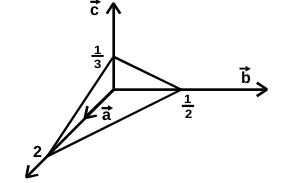
\includegraphics[width=0.9\textwidth]{abbildungen/miller_ind.png}
  \caption{Veranschaulichung einer Netzebene mit Miller-Indizes (1 4 6).\cite{sample}}
\end{figure}

Wie bereits erwähnt, haben benachbarte Netzebenen immer
den selben Abstand. Dieser Netzebenenabstand $d$ wird bei der
Strukturanalyse benötigt. In Abbildung \ref{fig:miller_abstand} wird
die Berechnung von $d$ veranschaulicht. Der Vektor, dessen Betrag $d$ ergibt,
muss einerseits orthogonal auf der eingezeichneten Netzebene und andererseits orthogonal
auf einer Benachbarten. Aus Überlegungen zu den in \ref{fig:miller_abstand}
eingezeichneten rechtwinkligen Dreiecken unter der Bedingung
\begin{align}
  \label{eqn:4}
  \cos\alpha^2 + \cos\beta^2 + \cos\gamma^2 = 1
\end{align}
lässt sich der Netzebenenabstand
durch
\begin{align}
  \label{eqn:5}
  d = \frac{a}{\sqrt{h^2 + k^2 + l^2}}
\end{align}
berechnen.

\begin{figure}[hhh]
  \centering
  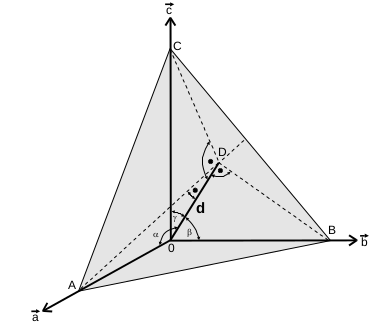
\includegraphics[width=0.9\textwidth]{abbildungen/miller_dist.png}
  \caption{Skizze zur Veranschaulichung der Berechnung des Netzebenenabstands.\cite{sample}}
\end{figure}

\subsection{Beugung von Röntgenstrahlung an Kristallen}
\label{subsec:Beugung}
Kristallstrukturen können mit Hilfe von Beugung
elektromagnetischer Wellen an Elektron und Atomkernen untersucht werden.
Dabei eignet sich Röntgenstrahlung für die Untersuchung, da diese Wellenlängen um
$\SI{1}{\angstrom}$ besitzt und somit in
die Größenordnung der Gitterkonstanten liegt.
Für die theoretische Beschreibung werden Elektron und Atomkernen
als Hertzsche-Dipole betrachtet, die mit einem
elektrischen Feld wechselwirken.
Für die Intensität eines punktförmiges Streuzentrum mit
Ladung $ze_0$ ergibt sich
\begin{align}
  I(r,\theta,z) = I_0\left(\frac{\mu_0 (ze_0)^2}{4\pi zm_0}\right)\frac{1}{r^2}\frac{1+\cos^2 2\theta}{2}=z^2 I_e \label{6}.
\end{align}
Durch die endliche Ausdehnung der Elektronenhülle,
müssen jedoch Phasenunterschiede
\begin{align*}
  \Delta\phi=2\pi\frac{\Delta s}{\lambda}= 2\pi\vec{r}\left(\vec{k}-\vec{k}_0\right)
\end{align*}
zwischen den gebeugten
Strahlen berücksichtigt werden und es wird
der Atomformfaktor $f$ als Quotienten
von am Atom gestreuter Intensität $I_a$ und $I_e$ der
Intensität eines Einzelelektrons
\begin{align}
f^2=\frac{I_a}{I_e}
\end{align}
von eingeführt.

Ebenfalls kann der Atomformfaktor $f$ als Fourier-Transformierte
der Ladungsverteilung $\rho(\vec{r})$
\begin{align}
f=\int_{\mathrm{Hülle}}
\symup{e}^{-\symup{i}\pi\Delta\phi}
\rho\left( \vec{r}\right) \symup{d}^3 r
 = \int_{\mathrm{Hülle}}
 \symup{e}^{-2\pi\symup{i}
 \left(\vec{k}-\vec{k}_0\right)}
 \rho\left( \vec{r}\right) \symup{d}^3 r
\end{align}
angesehen werden.
Somit ergibt sich die Streuamplitude
\begin{align}
  I_\mathrm{a}=f^2\left(z,\frac{\sin\theta}{\lambda}\right)I_\mathrm{e}\left(r,\theta\right)
\end{align}
eines Atome.
Die Streuamplitude $S$ einer Elementarzelle resultiert aus
phasenrichtiger Aufsummation der
einzelnen Atomstreuamplituden, wobei unterschiedliche
Atome an den Orten $\vec{r_j}$
andere Formfaktoren $f_j$ besitzen.
Somit folgt für die Streuamplitude oder auch Strukturamplitude genannt
\begin{align}
  S=\sum_j \symup{e}^{-2\pi \symup{i} \vec{r}_j\left(\vec{k}-\vec{k}_0\right)} I_\mathrm{e}.
\end{align}
Die Streuung findet nicht nur an
einer Elementarzelle statt, sondern an
Ebenenscharen im Kristall statt.
Wird dies berücksichtigt, ergibt sich die
Braggsche Bedingung
\begin{align}
n\lambda= 2\symup{d}\sin{\theta} \ \ \ \ n=1,2\dots \label{eqn:10}
\end{align}
mit dem Ebenenabstand $d$ und Ein- und Ausfallwinkel $\theta$.
Jeder auftretende Reflex erfüllt diese Bedingung.
Durch die dazu äquivalente Form
\begin{align}
\vec{k}-\vec{k}_0=\frac{n}{|\vec{d}|}=\vec{g7}
\intertext{mit dem Reziprokengittervektor\footnote{Die Basisvektoren und Reziprokenbasisvektoren erfüllen die Relation $A_i*a_j=\delta_{ij}$}}
\vec{g}(hkl)=h\vec{A}+k\vec{B}+l\vec{C}
\end{align}
folgt für die Streuamplitude der $(hkl)$-Ebene
\begin{align}
  S=\sum_j \symup{e}^{-2\pi \symup{i}(x_jh+y_jk+z_jl)}  I_\mathrm{e}. \label{eqn:Streu}
\end{align}
Sind sowohl die Atomformfaktor $f_j$ und
die Positionen $\vec{r}_j$ der
Basis bekannt, ist durch diese
Gleichung festgelegt,
ob ein Reflex für die $(hkl)$-Ebene
beobachtet wird $S\neq0$ oder nicht $S=0$.
% erweiterung auf einheiets zelle
% -erweiterung auf gitter
% -> Braggbedingung an Netzebenen
% -> Strukturamplitude S
%
\subsection{Debye-Scherrer Methode}
\label{subsec:Methoden}
Um die Kristallstruktur eines Probematerials
zu ermitteln, wird bei der Debye-Scherrer Methode
das Probematerial mit monochromatischer
Röntgenstrahlung bestrahlt.
Hierbei ist die Probe kein
Einkristall, sondern eine
kristalline, fein pulverisierte Probe
in der die Mikrokristallorientierungen statistisch
über den ganzen Raumwinkel verteilt sind.
Dies erhöht die Wahrscheinlichkeit, dass
einige Mikrokristalle in Reflexionsstellung
befinden und ein Bragg-Reflex beobachtet wird.
Mit Hilfe eines
Zählrohr-Goniometers oder
eines Filmstreifens wird der Beugungswinkel $\theta$
bestimmt. Durch systematisches Probieren wird
jedem Beugungswinkel $\theta$ eine Netzebenenschar
${(\pm h \pm k \pm l)}$ zugeordnet und somit versucht
eine zu den Reflexen passende Kristallstruktur und
die Gitterkonstante $a$
zu ermitteln.
% \cite{sample})
